\documentclass[handout]{beamer}
%\documentclass[•]{beamer}
\usepackage[latin1]{inputenc}
\usepackage{amsmath}
\usetheme{Luebeck}
\setbeamertemplate{footline}[frame number] 
\setbeamertemplate{navigation symbols}{} 
\usepackage{graphicx}
\usepackage{caption}
\usepackage{subcaption}
\usepackage{multirow} %Mulitrow tabels
\usepackage{array}

\graphicspath{{plots/}}


\title{Search for Dark Matter in the Upgraded High Luminosity LHC at CERN}
\subtitle{Sensitivity of ATLAS phase II upgrade to dark matter production}

\author{Sven-Patrik Hallsj\"{o}}
%\date{\today} 
\begin{document}
%\renewcommand*{\inserttotalframenumber}{\pageref{lastframe}}
\begin{frame}
\titlepage
\end{frame}


%Introduction.

\begin{frame}[shrink=10]\frametitle{Introduction}
\begin{block}{Who am I?}
\begin{itemize}
\item 5th year Y-programme student.
\item Defending a 30hp Masters thesis in applied physics.
\end{itemize}
\end{block}
\begin{block}{Project}
\begin{itemize}
\item The theses work was performed at Stockholm University. It started January 7th and ended May 16th (19 weeks).
\item The work was done with the ATLAS group at the University looking at the sensitivity for dark matter production after the phase II upgrade.
\end{itemize}
\end{block}
\end{frame}

\begin{frame}[shrink=10]\frametitle{Goals}
\begin{block}{}
\begin{itemize}
\item Compare observables before and after smearing. What observables are the least/most affected?	
\item Implement selection criteria that select the signal collisions efficiently while significantly reduce the background. 
\item Calculate the figure of merit $p$ for the given selection criteria before and after smearing.
\item Investigate other selection criteria and observables, to mitigate the effect of high luminosity. Use $p$ to rank different criteria after smearing.
\item Conclude on the effect of the high luminosity on the sensitivity for dark matter and possible ways to mitigate its effects using alternative observables and selection criteria. 
\end{itemize}
\end{block}
\end{frame}

\begin{frame}[shrink=10]\frametitle{Dark matter}
\begin{block}{What is dark matter?}
\begin{itemize}
\item Looking outside of our solar system it is seen that the rotational speed of galaxies does not increase, as expected, with distance to the rotational center, it is instead constant.
\item Dark matter is the name given to, among other things, one solution to the discrepancies of galactic rotations.
\end{itemize}
\end{block}
\begin{block}{Properties}
All that is known so far is given in the name Dark matter.
\begin{itemize}
\item Dark, no electromagnetic interaction.
\item Matter, have gravitational interactions.
\end{itemize}
It is known that it can not be made up by anything in the standard model of particle physics, thus a new physical description is needed to explain dark matter.
\end{block}
\end{frame}

\begin{frame}[shrink=10]\frametitle{Dark matter}
\begin{block}{}
There are several strategies to search for dark matter, the main one in this thesis is:
\begin{itemize}
\item Ordinary matter interacting with ordinary matter can produce dark matter, known as production. This is the process which occurs in particle accelerators and is the method explored in this thesis.
\end{itemize}
\end{block}
\end{frame}

\begin{frame}[shrink=10]\frametitle{LHC}
\begin{block}{}
The large hadron collider (LHC) is a particle accelerator located at CERN near Geneva in Switzerland. 
\end{block}
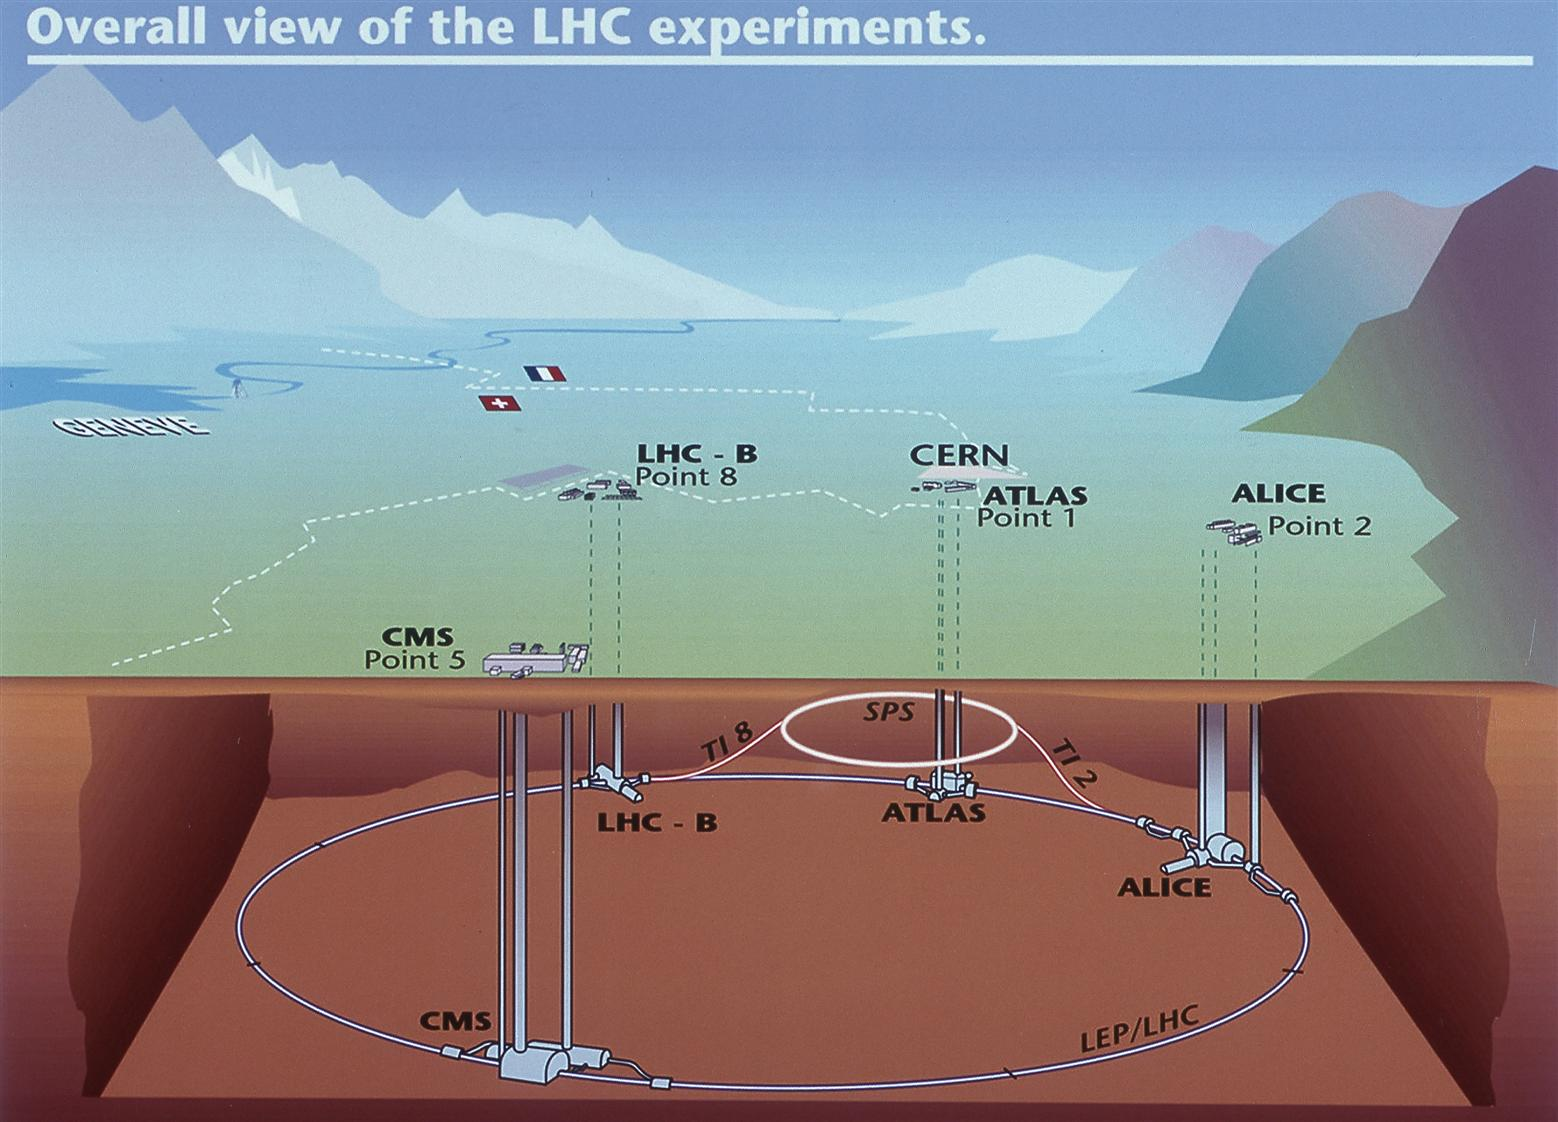
\includegraphics[scale=0.35]{lhc.jpeg}
\end{frame}

\begin{frame}[shrink=10]\frametitle{ATLAS}
\begin{block}{ATLAS}
The ATLAS detetor is a general purpose detector that uses a toroid magnet. Its goal is to observe several different production and decay channels
\end{block}
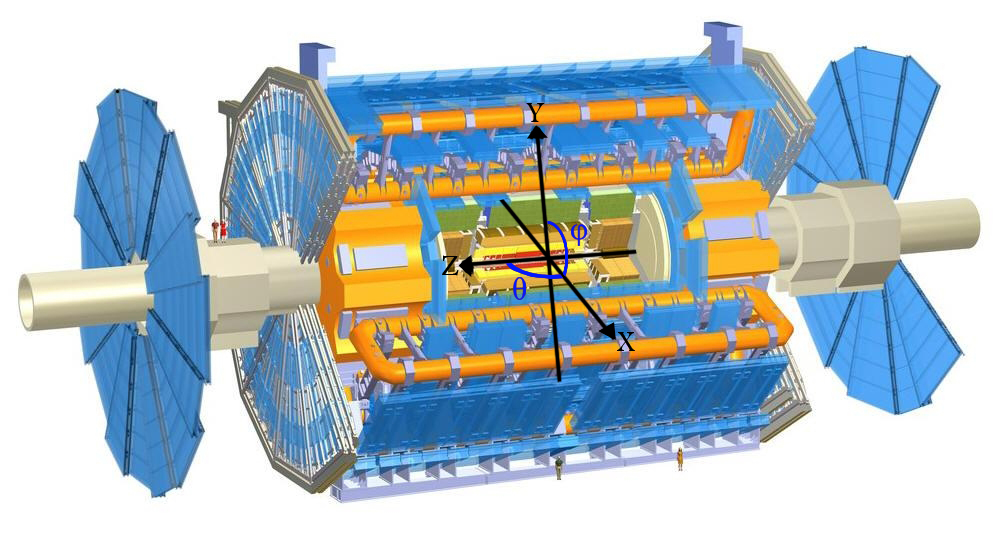
\includegraphics[scale=0.3]{particle_collider.jpg}
\end{frame}

\begin{frame}[shrink=10]\frametitle{Dark matter in particle collisions}
\begin{block}{}
\begin{itemize}
\item There are two main classes of events, signal and background. 
\item The signal corresponds to events that would arise from one of the DM processes.
\item It will not be possible for the ATLAS detector to directly detect dark matter signals, it will only be detected as missing energy through a mono-jet analysis.
\item ATLAS has looked at proton-proton collisions, with 8 TeV center of mass energy, $\sqrt{s}$, which contain high energetic jets without finding any excess of mono-jet events.
\item What is a mono-jet analysis?
\end{itemize}
\end{block}
\end{frame}

% However to know that the missing energy is a sign of the signal then one must understand all the other components that could contribute to the missing energy. Also there must be an excess of missing energy from what is expected from the background, since is it comprised of standard model processes that can mimic the mono-jet signature.

\begin{frame}[shrink=25]\frametitle{Mono-jet event}
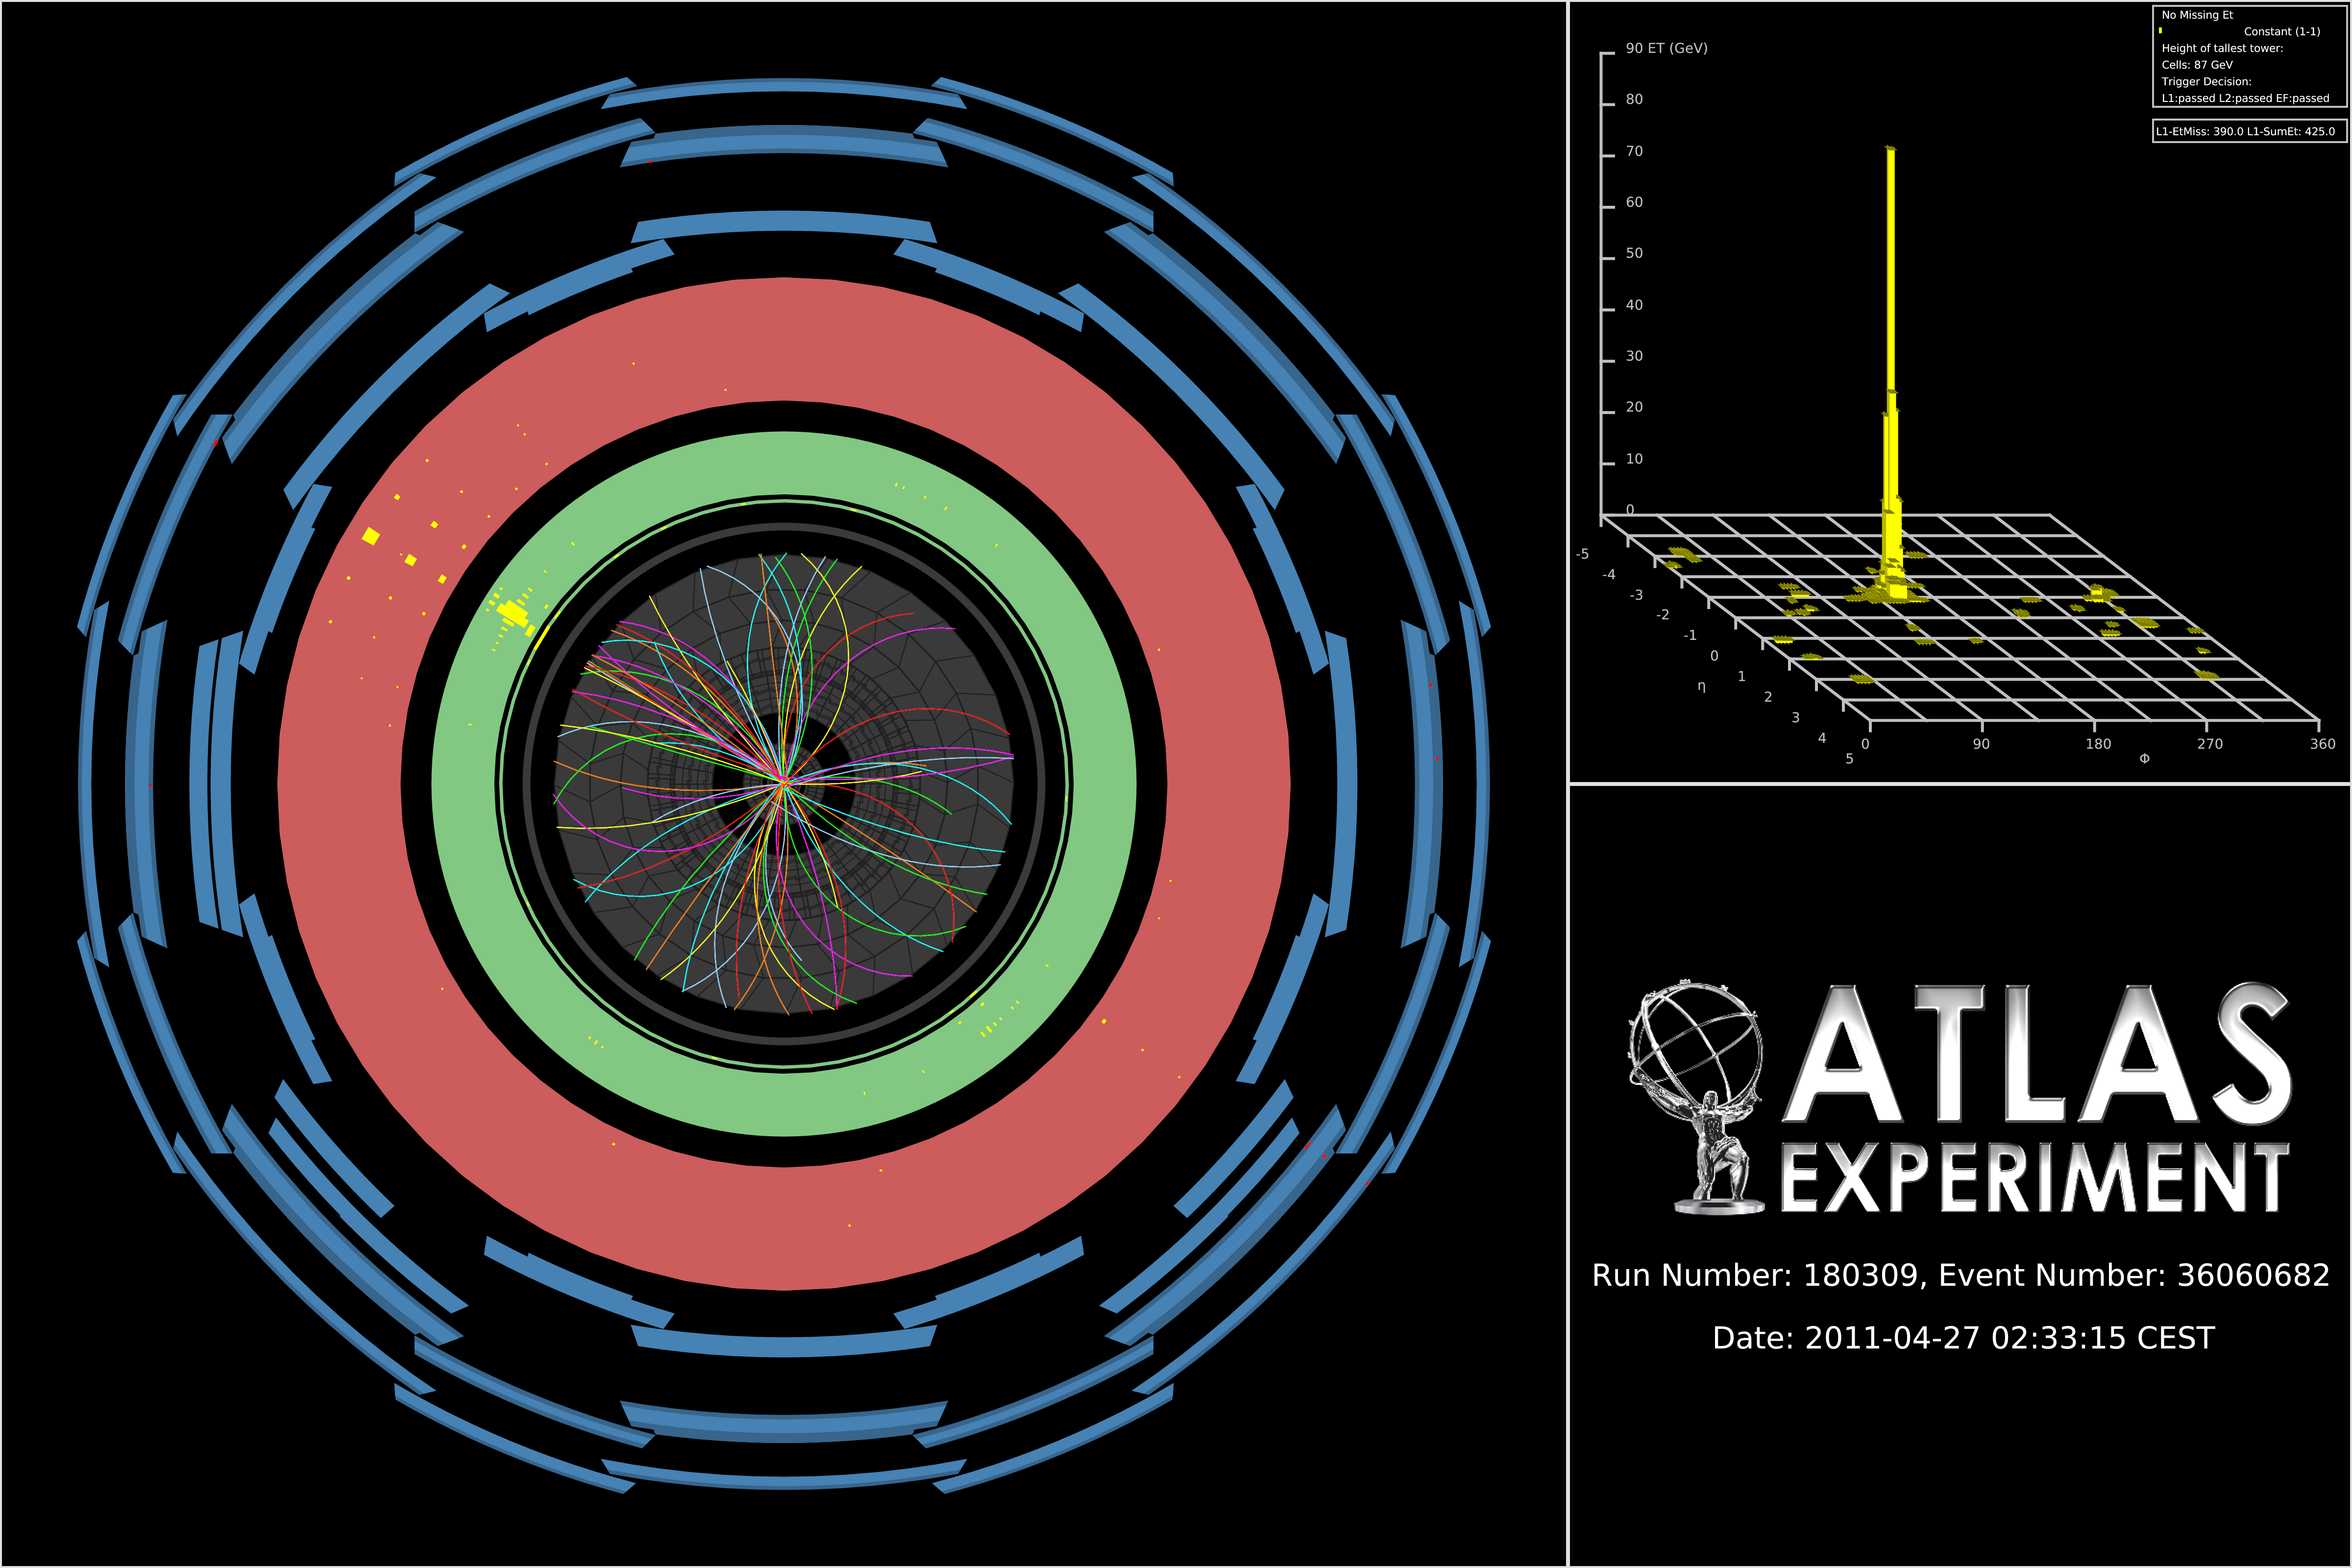
\includegraphics[scale=0.07]{monojetbig.png}
\begin{block}{}
Image in the transverse plane of a mono-jet event recorded by the ATLAS experiment. The figure in the top right is a diagram in the $(\eta,\varphi)$-plane showing where in the calorimeter (red in the main figure) the energy is deposited and how much.
\end{block}
\end{frame}

\begin{frame}[shrink=10]\frametitle{Mono-jet analysis}
\begin{block}{}
\begin{itemize}
\item Conservation of momentum in the transverse plane of the experiment indicates that the sum of all momenta should be zero as before the collision.

\item Since there is no balancing jet there must be transverse energy that is not detected, denoted $E_T^{Miss}$, indicating that the energy to balance this can not be detected. This could for instance be the characteristic signature of dark matter.
\end{itemize}
\end{block}
\begin{block}{Definition of $E_T^{Miss}$}
$E_T^{Miss}$ is the modulus of the $\vec{E_T}^{Miss}$ vector which is defined as:
\begin{equation*}
\vec{E_T}^{Miss} = - \sum \vec{p_T}^{Jet} - \sum \vec{p_T}^{Electron} - \sum \vec{p_T}^{Muon} - \sum \vec{p_T}^{Tau} - \sum \vec{p_T}^{Photon}
\end{equation*}  
where $p_T$ denotes the transverse momenta and the superscripts denote the detectable particles in the detector.
\end{block}


\end{frame}

%Neutrinos escape the \abbrATLAS experiment without being detected, and in this thesis it is assumed that \abbrWIMPS pass through all the detectors without leaving any trace. Therefore \abbrWIMPS and neutrinos have the same detector signature. As seen in \sectionref{chap:sig:sec:res} the main background to the \abbrWIMP signal is the production of a Z-boson that in turn decays to two neutrinos mimicking the \abbrWIMP signature.


\begin{frame}[shrink=10]\frametitle{Phase II upgrade}
\begin{block}{}
At the moment, the whole LHC is undergoing a step by step upgrade program which will be finalized around 2022-2023, denoted the high luminosity upgrade, or HL-upgrade. The upgrade consists of different stages, meaning that the upgrade
will halt for periods so that experiments can take place.
\end{block}
\begin{block}{}
The upgrade in focus in this thesis is known as phase II and will be implemented between 2021 and 2022-2023. It will increase the center of mass energy for the colliding particles to 14 TeV and the rate at which these are collided. The amount of data collected will also increase to $1000 fb^{-1}$.
\end{block}
\begin{block}{}
The increase in collision events, instantaneous luminosity [$fb^{-1}s^{-1}$, \\ 1 barn($b$)$= 10^{24} cm^2$], will unfortunately lead to events occurring simultaneously known as pile-up.
\end{block}
\end{frame}

\begin{frame}[shrink=10]\frametitle{Simulation of particle collisions}
\begin{block}{}
For the phase II upgrade there does not exist a full simulation of the detector. This thesis instead uses data from Monte Carlo simulations for the particle collisions and then uses so called smearing functions to emulate the detector responses.
\end{block}
\begin{block}{}
\begin{itemize}
\item The MC simulation, based on probability calculation from quantum mechanics, is denoted as truth data.
\item Data after the smearing is denoted reconstructed data or reco data and would be compared to measured data if there were any.
\end{itemize}
\end{block}
\end{frame}


%Introduction done.
%Validation.

\begin{frame}[shrink=10]\frametitle{Validation of smearing functions}
\begin{block}{}
\begin{itemize}
\item The smearing functions are the official functions developed from previous studies by the ATLAS collaboration for the study of the ATLAS phase II upgrade. 
\item The key result of those studies was that the direction of the momenta is unaffected and that only jets and $E_T^{Miss}$ are affected by pile-up.
\item Since this was confirmed in previous studies it was not incorporated into the smearing functions.
\item The first step of the project was to validate that these functions were implemented and functioned correctly.
\end{itemize}
\end{block}
\end{frame}

\begin{frame}[shrink=10]\frametitle{Smearing functions}
\begin{block}{}
\begin{itemize}
\item In a simulation of a proton-proton collision all quantities such as energy, momentum and direction of all produced particles are perfectly known. 
\item In a real experiment it is only possible to get measured values from the detector. 
\item The detector energy and momentum resolutions given in the smearing functions relate the measured values to the truth values on a statistical basis as given below.
\end{itemize}
\begin{equation*}
E' = E + \Delta E = E + \sigma
\end{equation*}
where $E$ is the energy at a truth level and $E'$ is the smeared energy and $\Delta$E or $\sigma$ is a random number obtained by sampling a Gaussian distribution with mean value 0 and a standard deviation equal to the resolution for that particle, and will be denoted $\sigma$.
\end{block}
\end{frame}

\begin{frame}[shrink=10]\frametitle{Validation}
\begin{block}{}
Since part of this thesis work is to take the official atlas smearing functions and apply the smearing to each particle, it is important to check that the energy and momenta resolutions of the smeared objects are consistent with the expected measured values. 
\end{block}
\end{frame}

\begin{frame}[shrink=10]\frametitle{Validation}
\begin{block}{}
In \ref{fig:tau:1} the Gaussian fit (red) and the data (black) are given for tau detected through 3 prong. In \ref{fig:tau:2} smeared energy is plotted against truth energy. 
\end{block}
\begin{figure}
        \centering
        \begin{subfigure}[b]{0.45\textwidth}
                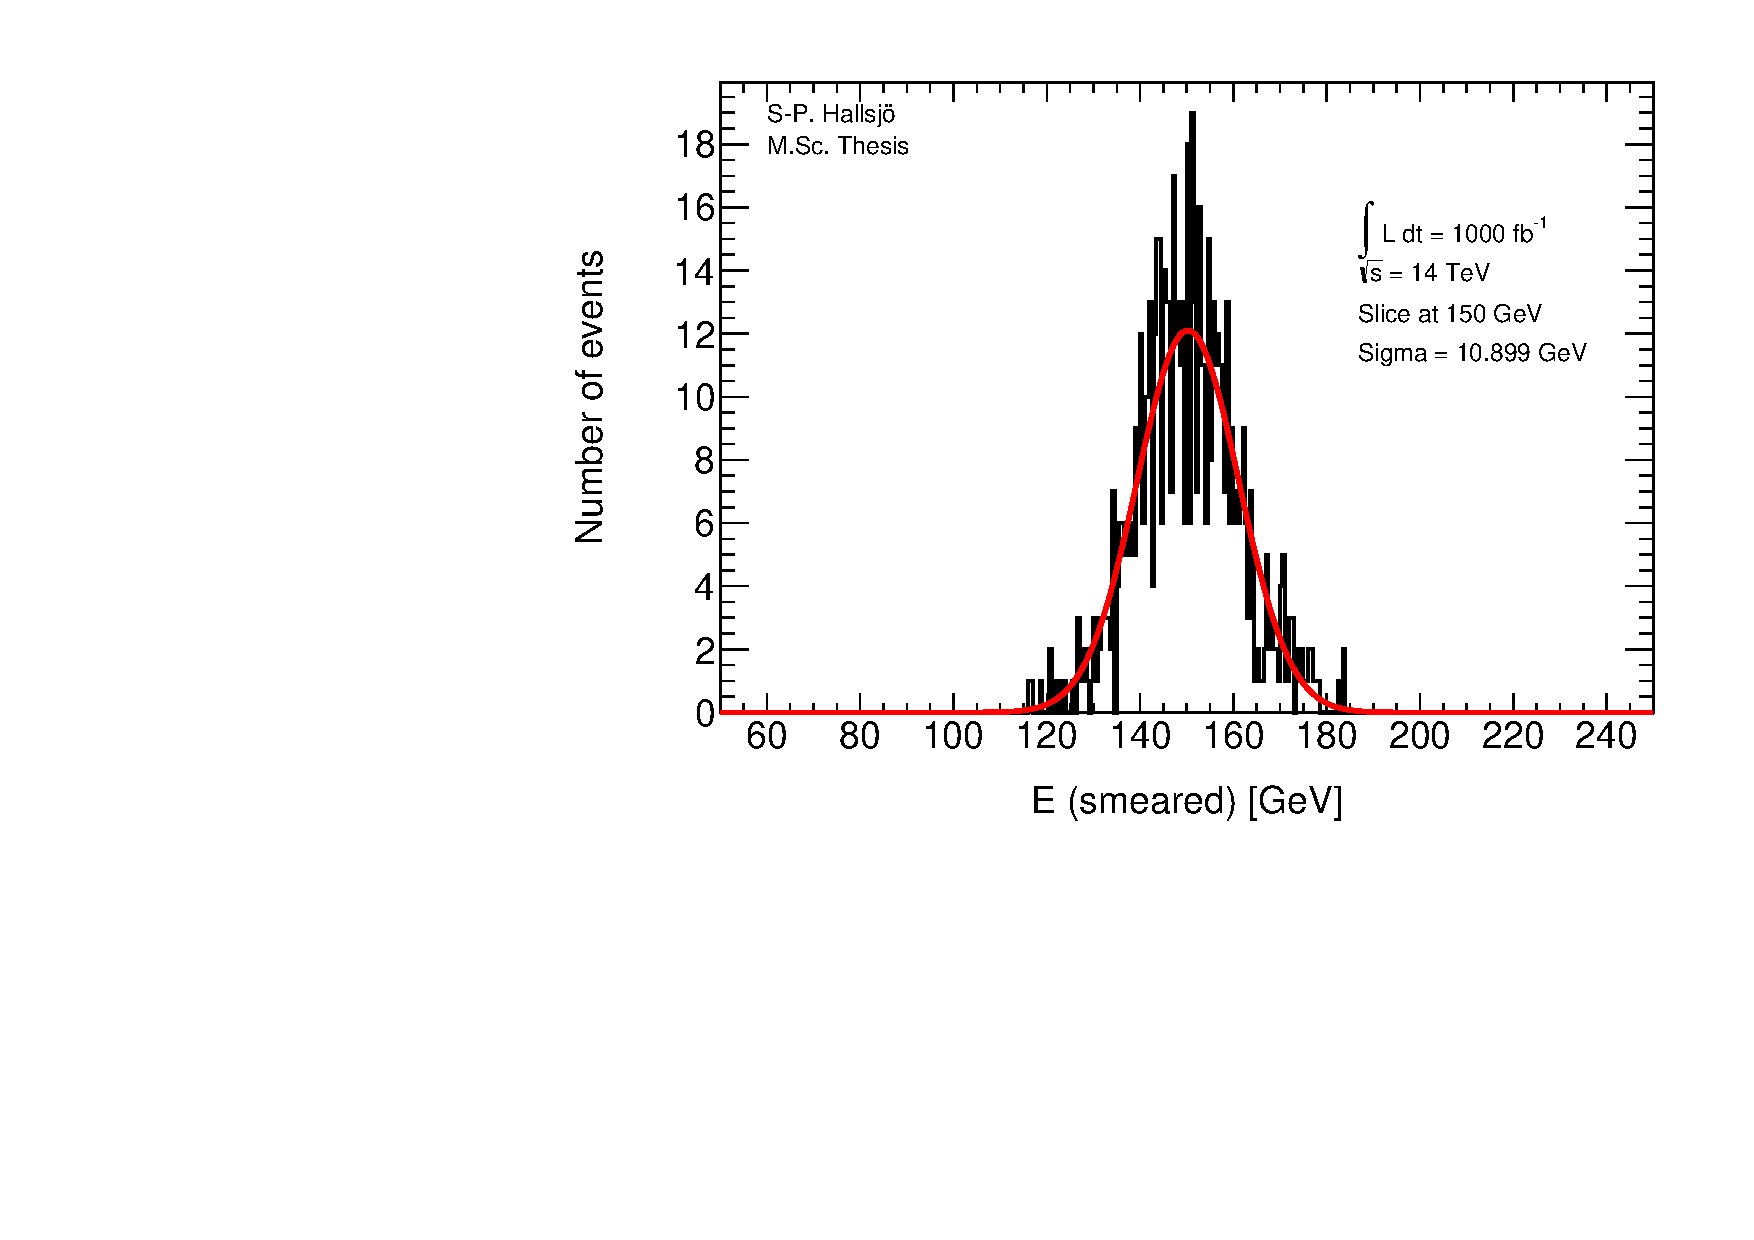
\includegraphics[width=\textwidth]{tau.pdf}
                \caption{Tau energy after smearing.}
                \label{fig:tau:1}
        \end{subfigure}
        \hfill
        \begin{subfigure}[b]{0.45\textwidth}
                 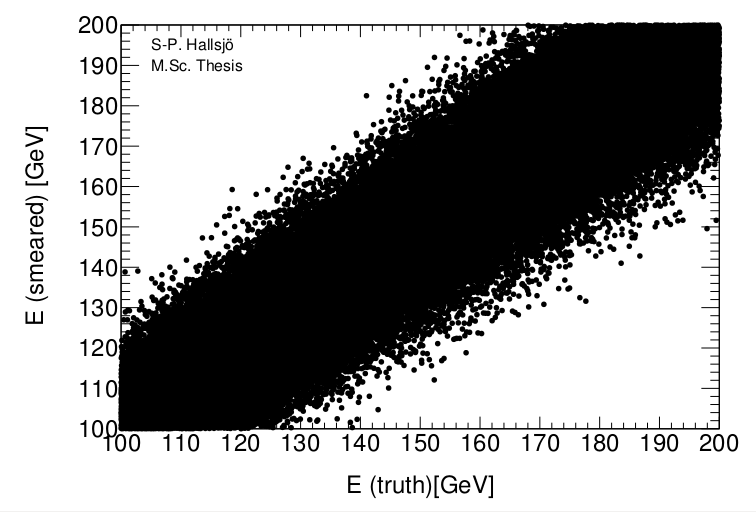
\includegraphics[width=\textwidth]{tau2.png}
                \caption{Tau smeared vs truth.}
                \label{fig:tau:2}
                 \end{subfigure}
    \caption{Tau energy after smearing and smeared vs truth.}
    \label{fig:tau}
           
\end{figure}

\end{frame}

\begin{frame}[shrink=10]\frametitle{Conclusion}
\begin{block}{}
The smearing functions work as intended within 5.8 sigma, however when using a test box and averaging the sigmas one ends up with half of this for the extreme
cases, muons and $E_T^{Miss}$. This indicates that the statistical fluctuation of these values and of the error calculations are considerable. Even with this statistical fluctuation the smearing functions work as intended.
\end{block}
\end{frame}

%Validation done.
%Dark matter.

\begin{frame}[shrink=10]\frametitle{Sensitivity to dark matter signals}
\begin{block}{Main part of the project}
With the validation completed focus turned to investigating the signal models. The following tasks were set and performed.
\begin{itemize}
\item Compare background simulation to previous measured data.
\item Evaluate the limit of the mass suppression scale of the D5 operator model.
\item Evaluate the limit of the mediator mass of the light vector mediator model. 
\end{itemize}
\end{block}
\end{frame}

\begin{frame}[shrink=10]\frametitle{Comparing events}
\begin{block}{Signal regions}
\begin{itemize}
\item To compare data, signal regions are used.
\item These are restrictions on certain parameters to minimize unwanted data. These are not known a priori and must be designed depending on what is interesting.
\end{itemize}
\end{block}
\end{frame}



\begin{frame}[shrink=20]\frametitle{Signal regions}
\begin{block}{}
The pre-selection criteria used in Ref. ATLAS-CONF-2012-147 are the following:
\begin{itemize}
\item Jet veto, require no more than 2 jets with $p_T > 30 GeV$ and $|\eta| < 4.5$.  \\ 
This is done to reduce the number of multi-jet events.
\item Lepton veto, no electron or muon. \\
These vetos are there to remove uninteresting $W \rightarrow e \nu$ and $W \rightarrow \mu \nu$ background events.
\item Leading jet with $|\eta| < 2.0$ and $\Delta \varphi (jet, E_T^{Miss})>0.5$ (second-leading jet).\\ 
This is done to further reduce the number of multi-jet events.
\end{itemize}
The following signal regions were used:
\end{block}
\begin{table}[h]
\renewcommand{\arraystretch}{1.2} %Change back
\begin{center}
\begin{tabular}{l l l l l l}
\hline
signal region & SR3p & SR4p \\ \hline
minimum leading jet p$_T$ (GeV) & 350 & 500 \\
minimum E$^{Miss}_T$ (GeV) & 350 & 500 \\ \hline
\end{tabular}
\label{tab:oldsr}
\caption{The signal regions from Ref. ATLAS-CONF-2012-147.}
\end{center}
\renewcommand{\arraystretch}{1.0} %Change back
\end{table}
\end{frame}



\begin{frame}[shrink=20]\frametitle{Signal regions}
\begin{block}{}
The proposed pre-selection criteria differ in the veto:
\begin{itemize}
\item Electron veto which is defined: $\Delta R (jet^{lead},electron^{lead})\geq 0.4$ and \\
$electron^{lead} p_T>20 GeV$ removed.
\item Muon veto which is defined: $\Delta R (jet^{lead},muon^{lead})\geq 0.4$ and \\
$muon^{lead} p_T>20 GeV$ removed. \\
These formulation of vetos are used to remove uninteresting $W \rightarrow e \nu$ and $W \rightarrow \mu \nu$ background events without removing too much of the signal. The $\Delta R$ involvement is to make sure that the veto is only on simulated true particles and not simulated false detections.
\end{itemize}
Here the superscript lead denotes the entity with highest transverse momentum $p_T$. Thus $electron^{lead}$ would be the simulated electron in an event with the highest $p_T$.
\end{block}
\end{frame}
\begin{frame}[shrink=20]\frametitle{Signal regions}
\begin{block}{}
To try and minimize the amount of background compared to the amount of signal, the following  signal regions are used:
\end{block}
\begin{table}[h]
\renewcommand{\arraystretch}{1.2} %Change back
\begin{center}
\begin{tabular}{l l l l l l}
\hline
Symmetric signal region & SR1 & SR1p & SR2 & SR3 & SR4 \\ \hline
minimum leading jet p$_T$ (GeV) & 350 &500& 600 & 800 & 1000 \\
minimum E$^{Miss}_T$ (GeV) & 350&500 & 600 & 800 & 1000 \\
\end{tabular}
\begin{tabular}{l l l l l} \hline
Asymmetric signal region & SRa &  SRb & SRc & SRd \\ \hline
minimum leading jet p$_T$ (GeV) & 350 & 350 & 350 & 350 \\
minimum E$^{Miss}_T$ (GeV) & 350 & 600 & 800 & 1000 \\ \hline
\end{tabular}
\caption{The new signal regions.}
\label{tab:newsr}
\end{center}
\renewcommand{\arraystretch}{1.0} %Change back
\end{table}
\end{frame}

\begin{frame}[shrink=20]\frametitle{Comparing with a previous paper}
\begin{block}{Comparison}
To make sure that the utilized background is correct, it is compared to the background from the article:\\
ATLAS-CONF-2012-147, Search for New Phenomena in Monojet plus Missing Transverse Momentum Final States using 10fb-1 of pp Collisions at $\sqrt{s}=8$ TeV with the ATLAS detector at the LHC. 
\end{block}
\begin{block}{}
For the comparison to be done, samples of data comparable to measured data needed to be used.
\end{block}
\end{frame}

\begin{frame}[shrink=33]\frametitle{Comparing with a previous paper}
\begin{table}[ht]
\begin{center}
\begin{tabular}{|l|l|l|l|l|}
\hline
& \multicolumn{2}{c}{SR3p} & \multicolumn{2}{|c|}{SR4p} \\
\hline
Process & Work & Paper & Work & Paper \\ \hline
Z$\rightarrow\nu\nu$ & 140298 & 152000 & 25250 & 27000 \\
W$\rightarrow\tau\nu$ & 40701 & 37000 & 5862 & 3900 \\
W$\rightarrow e\nu$ & 11229 & 11200 & 1507 & 1600 \\
W$\rightarrow\mu\nu$ & 13727 & 15800 & 1872 & 4200 \\ \hline
Total background & 205955 & 218000 & 34491 & 36700 \\ \hline
\end{tabular}
\caption{Comparison of the simulated events with expected events from ATLAS-CONF-2012-147 with $L=1000$fb$^{-1}$, cross-sections corresponding to $\sqrt{s}=8$TeV and using the same electron and muon veto.}
\label{tab:Compare1}
\end{center}
\end{table}

\begin{table}[ht]
\begin{center}
\begin{tabular}{|l|l|l|l|l|}
\hline
& \multicolumn{2}{c}{SR1} & \multicolumn{2}{|c|}{SR1p} \\
\hline
Process & Work  & Paper & Work & Paper  \\ \hline
Z$\rightarrow\nu\nu$ & 150753 & 152000 & 27569 & 27000 \\
W$\rightarrow\tau\nu$ & 49320 & 37000 & 7318 & 3900 \\
W$\rightarrow e\nu$ & 18329 & 11200 & 2534 & 1600 \\
W$\rightarrow\mu\nu$ & 22290 & 15800 & 3218 & 4200 \\ \hline
Total background & 240690 & 218000 & 40639 & 36700 \\ \hline
\end{tabular}
\caption{Comparison of the simulated events with expected events from ATLAS-CONF-2012-147 with $L=1000$fb$^{-1}$, cross-sections corresponding to $\sqrt{s}=8$TeV and using a modified electron and muon veto.}
\label{tab:newcomp}
\end{center}
\end{table}
\end{frame}

\begin{frame}[shrink=0]\frametitle{Conclusion from comparison}
\begin{block}{Background}
\begin{itemize}
\item The background is similar.
\item $\tau$ is higher since there is no way for $\tau$ to be reconstructed as jets in the code, with the cut above this will have a large impact. $\phi (second leading jet, E_T^{miss})>0.5$
\item The veto needed to change for the signal to survive.
\item In the proposed there is no veto on false detections.
\end{itemize}
\end{block}
\begin{block}{}
Since the background is validated, the signals can be evaluated.
\end{block}
\end{frame}




\begin{frame}[shrink=10]\frametitle{Compare signal to background}
\begin{block}{Sensitivity}
\begin{itemize}
\item Measured as the probability of having the background fluctuate to S+B.
\item If p $<0.05$ then we have sensitivity.
\end{itemize}
\end{block}
\begin{block}{}
To compute sensitivity at 14 TeV need to make assumptions about uncertainties in the background events.

Use 10 fb$^{-1}$ mono-jet paper as baseline.  
\begin{itemize}
\item In total the error is either, 0.08 or 0.02.
\end{itemize}  
\end{block}
\end{frame}



\begin{frame}[shrink=10]\frametitle{D5 operator model}
\begin{block}{D5}
The operator is based on the assumption that the mediator between dark matter and ordinary mater acts like a heavy z-boson.
\end{block}
\begin{block}{Mass suppression scale limit}
The cross-section, related to the probability of the process is scaled for D5 using M* as, $\sigma (M*) = (\frac{\sigma_{ref}}{M*})^4$ where $\sigma_{ref}$ is the theoretically calculated value.

The goal is to find the value of M* for which p=0.05 when compared to the background.
\end{block}
\begin{block}{Available models}
Two different models, one with an assumed dark matter mass of 50 GeV and the other at 400 GeV are evaluated.
\end{block}
\end{frame}

\begin{frame}[shrink=10]\frametitle{D5 operator model}

\begin{figure}
        \centering
        \begin{subfigure}[b]{0.45\textwidth}
                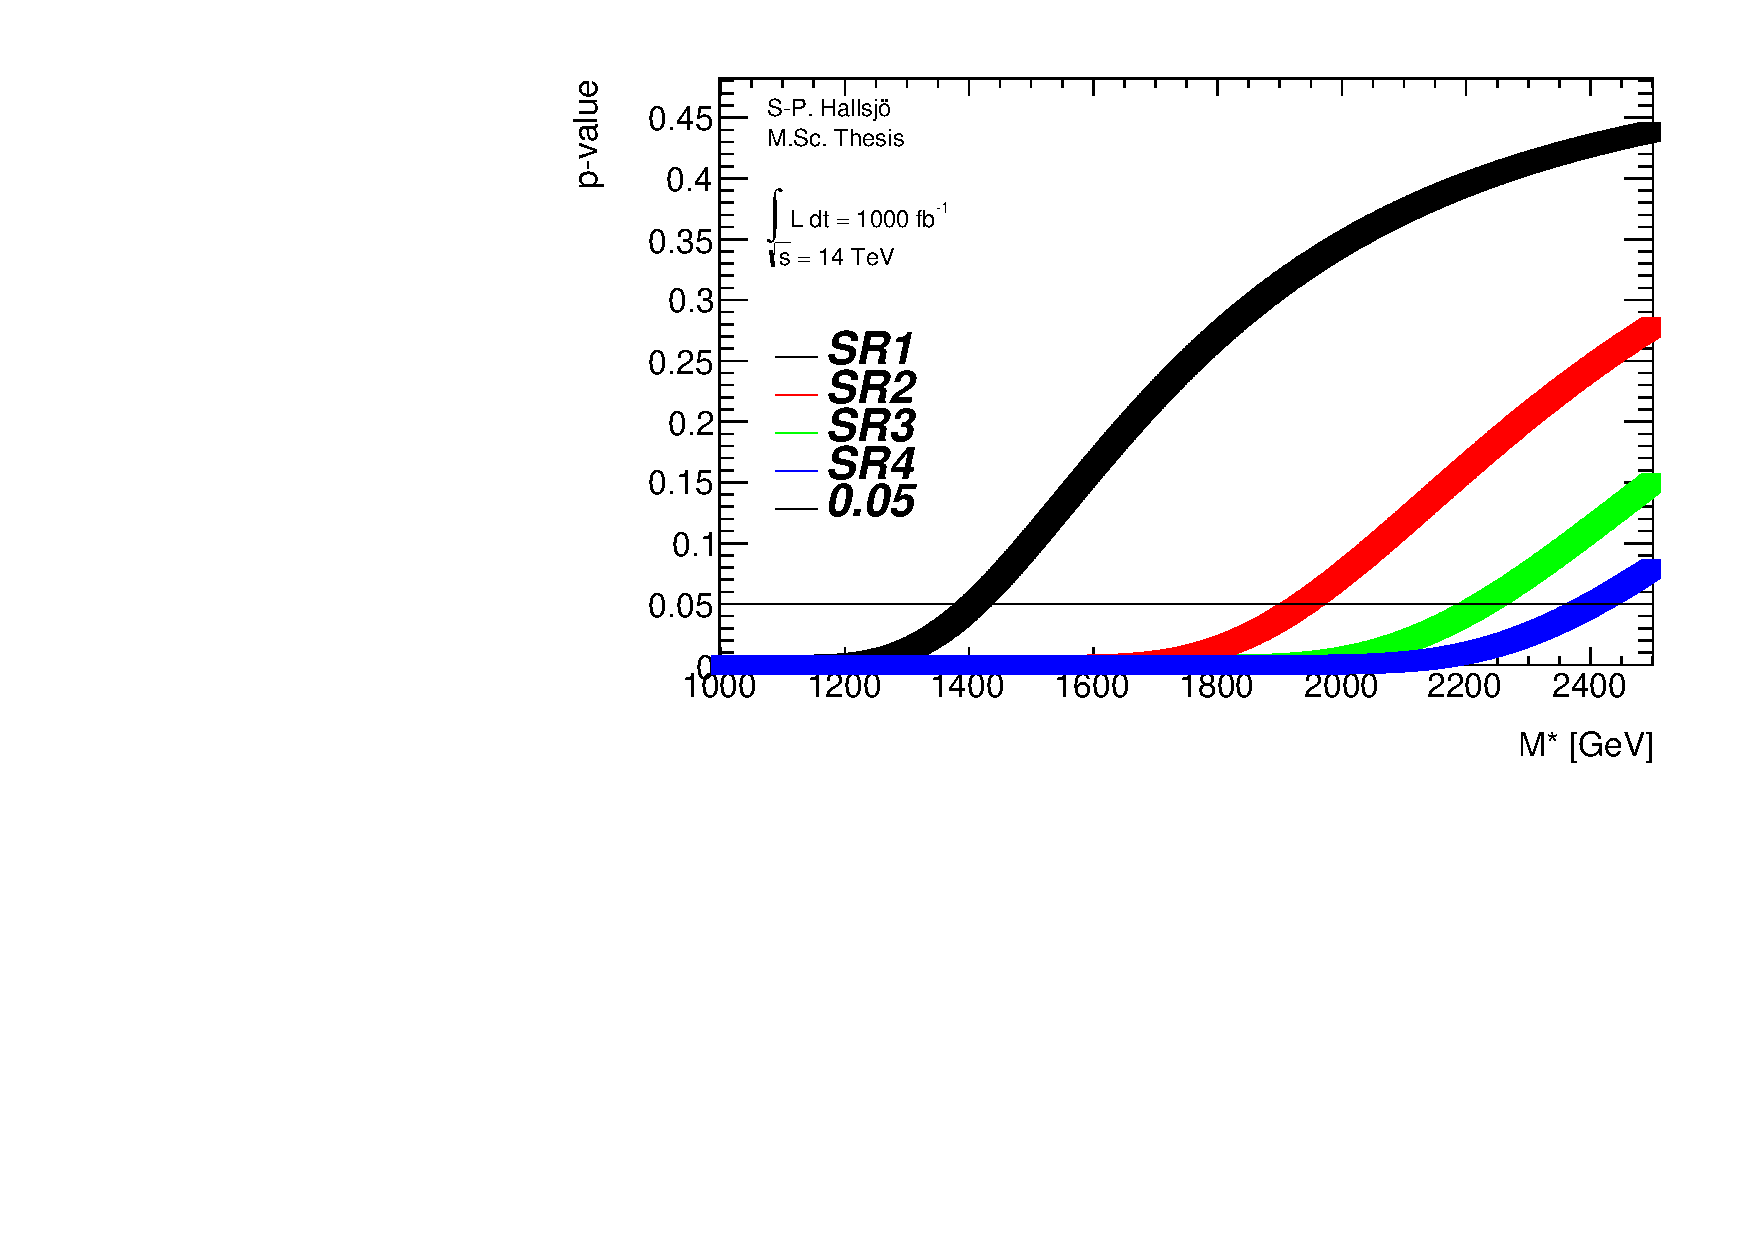
\includegraphics[width=\textwidth]{pvald5002truth2.pdf}
        
        \end{subfigure}
        \hfill
        \begin{subfigure}[b]{0.45\textwidth}
                 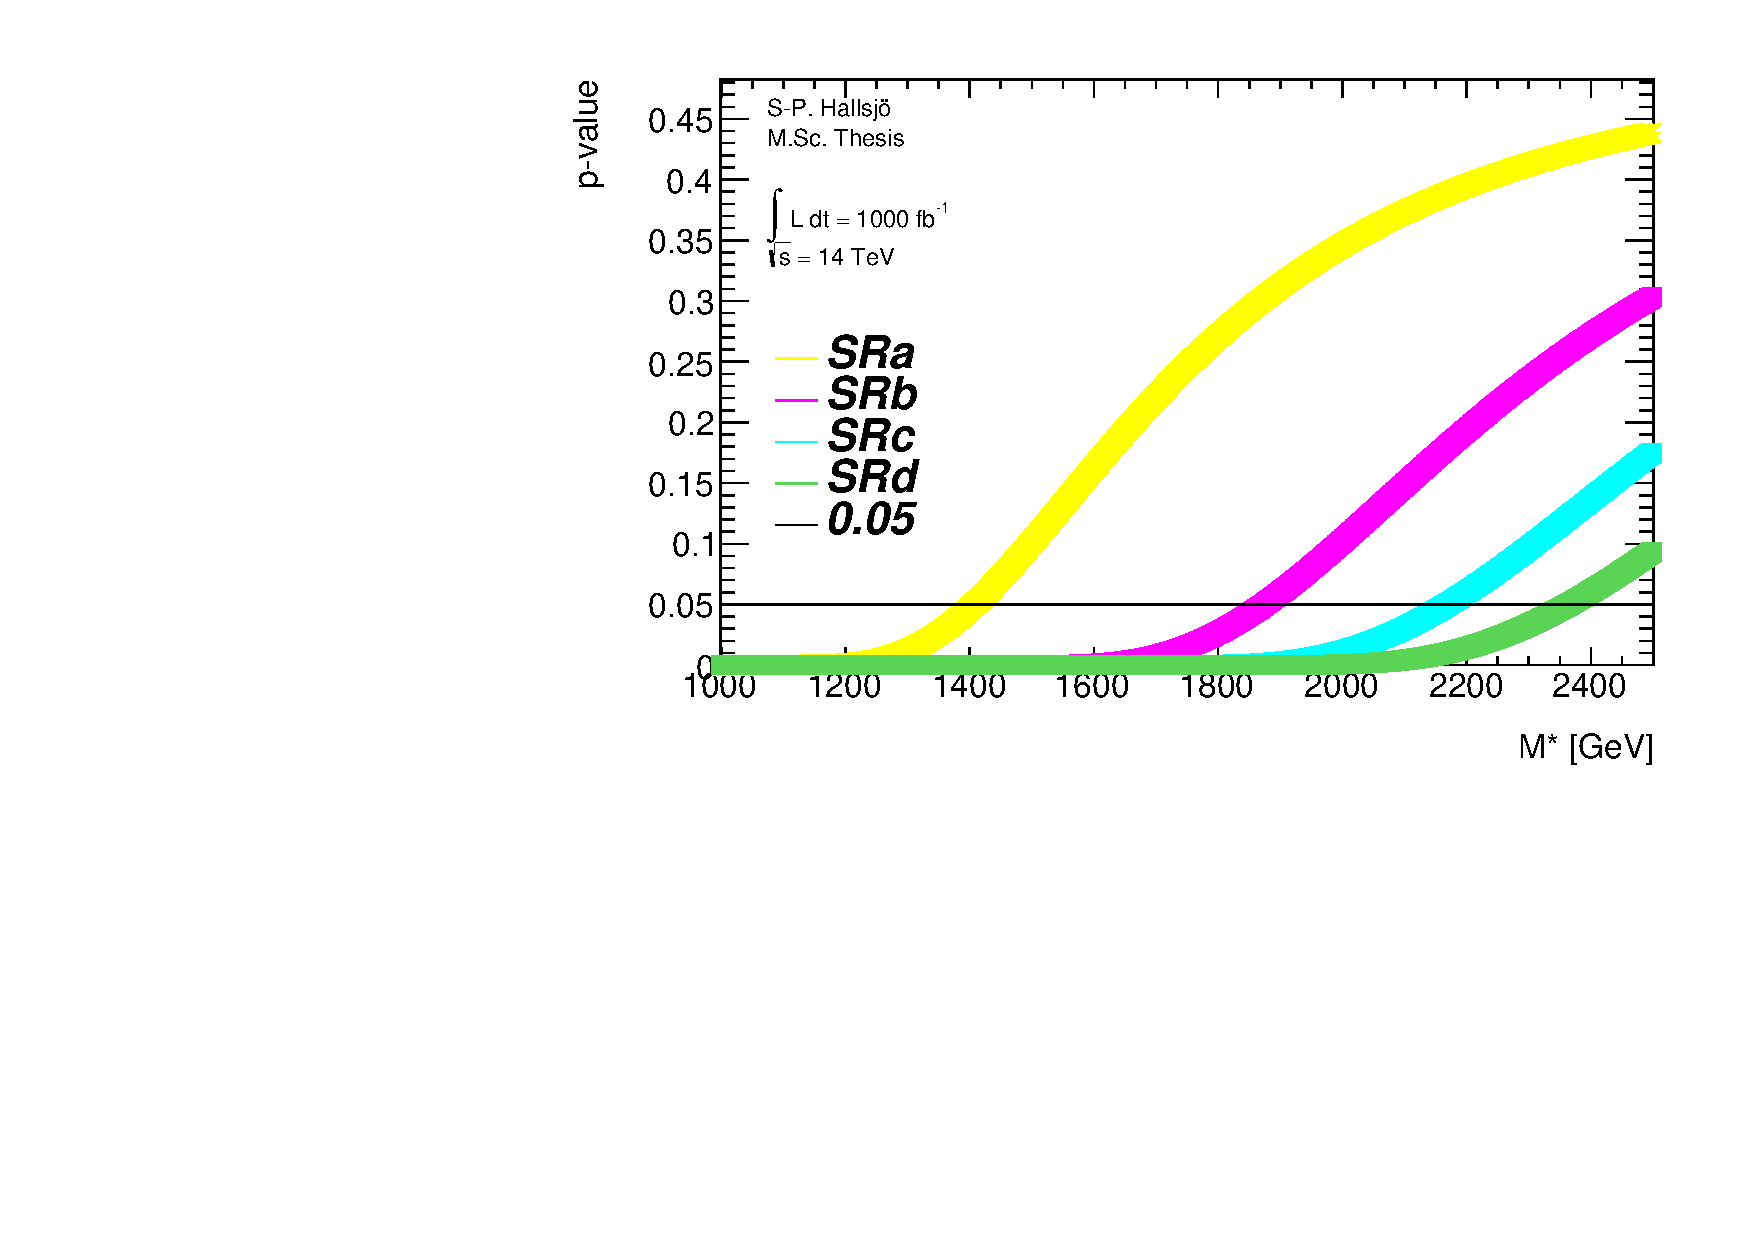
\includegraphics[width=\textwidth]{pvald5002truth.pdf}
    
             
                 \end{subfigure}
    \caption{p-value as a function of the mass suppression scale M* at truth level for error model 0.02.}
             
\end{figure}
\end{frame}


\begin{frame}[shrink=10]\frametitle{Conclusion}
\begin{block}{}
Increasing the centre of mass energy will increase the limits by a factor of 2-3.
\end{block}


\begin{table}[ht]
\begin{center}
\begin{tabular}{|l|l|l|}
\hline
Dark matter mass & From simulation & From paper \\ \hline
50 GeV & 1960 GeV &800 GeV \\
400 GeV & 1871 GeV & 700 GeV \\ \hline
\end{tabular}
\caption{M* values in SR2 from both simulation at 14 TeV, 1000fb$^{-1}$ and from 8 TeV and 10fb$^{-1}$. }
\label{Comp pval}
\end{center}
\end{table}
\end{frame}

\begin{frame}[shrink=10]\frametitle{Light vector mediator model}
\begin{block}{Models}
In this thesis these signals have two different width scenarios, $M$/3 and $M$/8$\pi$ where $M$ denotes the mediator mass. The width scenarios contain eight different mediator mass scenarios with masses between 100 and 15000 GeV. In addition to this there are, as with the D5 operator, two different dark matter masses, one at 50 GeV and one at 400 GeV.
\end{block}
\end{frame}
\begin{frame}[shrink=10]\frametitle{Light vector mediator model}
\begin{table}[ht]
\begin{center}
\begin{tabular}{|l|l|l|}
\hline
width & $m_{\chi}=50$ GeV & $m_{\chi}=400$ GeV \\ \hline
M/3 & 1000 GeV & 1000 GeV \\ \hline
M/$8\pi$ & 3000 GeV & 3000 GeV\\ \hline
\end{tabular}
\caption{Limits on the highest mediator mass model which can be excluded for different widths, different dark matter masses for truth and reconstructed data and both error models in SR2, 3, 4, c, d.}
\label{tab:mediatorpass}
\end{center}
\end{table}
\begin{table}[ht]
\begin{center}
\begin{tabular}{|l|l|l|}
\hline
width & $m_{\chi}=50$ GeV & $m_{\chi}=400$ GeV \\ \hline
M/3 & 1000 GeV & 1000 GeV\\ \hline
M/$8\pi$ & 1000 GeV & 1000 GeV\\ \hline
\end{tabular}
\caption{Limits on the highest mediator mass model which can be excluded for different widths, different dark matter masses for truth and reconstructed data and both error models in SRb.}
\label{tab:mediatorpass2}
\end{center}
\end{table}
\end{frame}

%Dark matter done.

\begin{frame}[shrink=10]\frametitle{Final conclusion}
\begin{block}{Limit on M*}
The limits can be found in subsection 3.3.3 and are 2-3 times better than previous
results at 8 TeV and 10fb$^{-1}$.
\end{block}
\begin{block}{Limit on mediator mass models}
The limits are found in the previous slide and are the first result done with these models and thus can not be compared.
Effect of the high luminosity
\end{block}
\begin{block}{Pile-up}
The effect of increased pile-up is at most $<$ 5\% compared to truth level on the mass suppression scale and does not affect the vector mediator models limits.
\end{block}
\end{frame}

\begin{frame}[shrink=10]\frametitle{Final remarks}
\begin{block}{}
The most interesting continuation of this work would be to compare the results given here to measurements done after the phase II upgrade, and hopefully see characteristic signatures from dark matter.
\end{block}
\end{frame}

\begin{frame}\frametitle{Thank you}
\begin{block}{}
Thank you for your attention.
\end{block}
\end{frame}


\begin{frame}[noframenumbering]\frametitle{Backup}

\end{frame}

\begin{frame}[shrink=10, noframenumbering]\frametitle{Summary of validation}
\begin{table}[H]
\begin{center}
\begin{tabular}{|l|l|l|l|l|}
\hline
Process& $\eta$ value & Pile-up value &$\sigma$ [GeV]& Expected $\sigma$ [GeV]\\ \hline
\multirow{2}{*}{Electron}& Low $\eta$&60&$1.25 \pm 0.05$&1.18\\
&High $\eta$&60&$1.82 \pm 0.14$&1.74\\ \hline
\multirow{2}{*}{Photon} & Low $\eta$&60&$1.19 \pm 0.04$&1.18\\
&High $\eta$&60&$1.80 \pm 0.04$&1.74\\ \hline
\multirow{2}{*}{Muon} & Low $\eta$&60&$1.19 \pm 0.05$&1.50\\
&High $\eta$&60&$1.71 \pm 0.09$&2.18\\ \hline
Tau& All $\eta$&60&$10.9 \pm 0.3$&10.3\\ \hline
\multirow{6}{*}{Jet} &Low $\eta$&60&$11.4 \pm 0.4$&11.6\\
&Low $\eta$&140&$15.4 \pm 0.5$&15.8\\
&Mid low $\eta$&60&$11.5 \pm 0.5$&11.9\\
&Mid low $\eta$&140&$15.1 \pm 0.7$&15.9\\
&Mid high $\eta$&60&$11.3 \pm 0.3$&10.9\\
&High $\eta$&60&$16.6 \pm 1.5$&13.5\\ \hline
\multirow{2}{*}{$E_T^{Miss}$}&All $\eta$&60&$43 \pm 2$&48\\ 
&All $\eta$&140&$105 \pm 12$&87\\  \hline
\end{tabular}
\end{center}
\caption{Calculated $\sigma$ values compared to $\sigma$ given from the resolution. Values are given at different pile-up values for comparison.}
\label{tab:sigmaval}
\end{table}
\end{frame}

\begin{frame}[shrink=10, noframenumbering]\frametitle{D5 operator model}
\begin{table}[ht]
\begin{center}
\begin{tabular}{|l|l|l|}
\hline
Signal region & Truth [GeV]& Reconstructed [GeV]\\ \hline
SR1, symmetric 350 GeV &1407&1402\\
SR2, symmetric 600 GeV&1936&1934\\
SR3, symmetric 800 GeV&2227&2226\\
SR4, symmetric 1000 GeV&2404&2406\\ \hline
SRa, asymmetric 350 GeV &1425&1421\\
SRb, asymmetric 600 GeV &1874&1803\\
SRc, asymmetric 800 GeV&2169&2125\\
SRd, asymmetric 1000 GeV&2365&2340\\ \hline
\end{tabular}
\caption{Limits on mass suppression scales in GeV given for $m_{\chi}=50$ GeV and the 0.02 error model.}
\label{tab:masssupp002}
\end{center}
\end{table}
\end{frame}
\begin{frame}[shrink=10, noframenumbering]\frametitle{D5 operator model}
\begin{table}[ht!]
\begin{center}
\begin{tabular}{|l|l|l|}
\hline
Signal region & Truth [GeV]& Reconstructed [GeV]\\ \hline
SR1, symmetric 350 GeV &1333&1329\\
SR2, symmetric 600 GeV&18481&1847\\
SR3, symmetric 800 GeV&2162&2163\\
SR4, symmetric 1000 GeV&2332&2303\\ \hline
SRa, asymmetric 350 GeV&1350&1346\\
SRb, asymmetric 600 GeV&1789&1721\\
SRc, asymmetric 800 GeV&2106&2059\\
SRd, asymmetric 1000 GeV&2288&2258\\ \hline
\end{tabular}
\caption{Limits on mass suppression scales in GeV given for $m_{\chi}=400$ GeV and the 0.02 error model.}
\label{tab:masssupp2002}
\end{center}
\end{table}
\end{frame}

\end{document}
